\documentclass[a4paper,11pt]{article}
\usepackage[utf8]{inputenc}
\usepackage[T1]{fontenc}
\usepackage[magyar]{babel}
\usepackage{geometry}
\geometry{a4paper, tmargin = 18mm,
lmargin = 25mm, rmargin = 25 mm, bmargin = 18 mm}
\usepackage{mathtools}
\usepackage{listings}
\usepackage{multirow}
\usepackage{setspace}
\usepackage{graphicx}
\usepackage{wrapfig}
\usepackage{enumitem}

\usepackage{listings}
\lstset{language=C}

\author{Nagy Kapolcs Ompoly}
\title{Arduino Clap Sensitive Light Control}
\date{ }
\linespread{1.42}
\begin{document}
\begin{titlepage}
	\centering
	
\includegraphics[width=0.15\textwidth]{eltecimer.jpg}\par
	\vspace{1cm}
	{\Large\itshape Mikrokontrollerek és alkalmazásaik Labor\par}
	{\huge\bfseries Arduino: \par Clap Sensitive Light Control\par}
	
	\vfill
	
	\raggedleft
	Beadás: 2019.05.17.\par
	\vspace{0.5cm}
	Nagy Kapolcs Ompoly\par
	(W7R17G)\par
	3. évfolyam\par
	Pénteki csoport\par
	
	\vspace{0.5cm}

	\centering
	{\small\itshape Félévi Projekt Jegyzőkönyv \par}
\end{titlepage}
\clearpage
\setcounter{page}{1}
\newpage
\renewcommand{\thesection}{\Roman{section}}
\renewcommand{\thesubsection}{\thesection.\arabic{subsection}}
\renewcommand{\thesubsubsection}{\thesubsection.\arabic{subsubsection}}
\section{Projektmunka célja}
A projekt célja, hogy mikrokontroller segítségével egy LED szalagot írányítsunk hangérzékelővel, mivel így 1 vagy 2 kézen kívül nincs szükség a több végtagra, hogy tudjuk kontrollálni a környezet fényforrásának az állapotát.

\section{Eszközök}

\begin{itemize}
	\item Uno R3 board + USB cable
	\item Uno R3 Extension board + GPIO Extension Board + Connecting Cable
	\item Breadboard + Jump Wires
	\item Sound Sensor Module 
	\item SS8050 NPN Transistor
	\item 12V LED strip
	\item 12v AC/DC LED Driver
\end{itemize}

\pagebreak

\section{Projektmunka}

\subsection{Megvalósítás}

A jelenlegi projektben azt szerettem volna elérni, hogy két egymásutáni tapsra fel illetve le tudjam kapcsolni a LED szalagot. Ehhez egy arduinos hang detektort használtam, aminek a digitális kimenetelét olvasom, ami a hang intenzitást figyeli és egy küszöbértékhez képest, vagy HIGH, vagy LOW értéket ad. Ezt int-é alakítva figyelem én is és abban az esetben, ha ez 1-el egyenlő, akkor elkezdem számolni, hány taps volt egymás után. Ez után 600 miliszekundumonként megnézem, hogy volt-e 2 taps és ha volt, akkor a led-et fel, vagy lekapcsolom az adott állapotához képest. 

A kód részéről ennyit, a áramkör megvalósításánál az volt az izgalmas számomra, hogy a LED szalagnak nem volt elég az 5V így külső áramforrással kellett megoldanom úgy, hogy egy tranzisztort kapcsolgatok illetve a hálozati áramot kellett 12V-á alakítani.

\subsection{Kapcsolási rajz}

\begin{center}
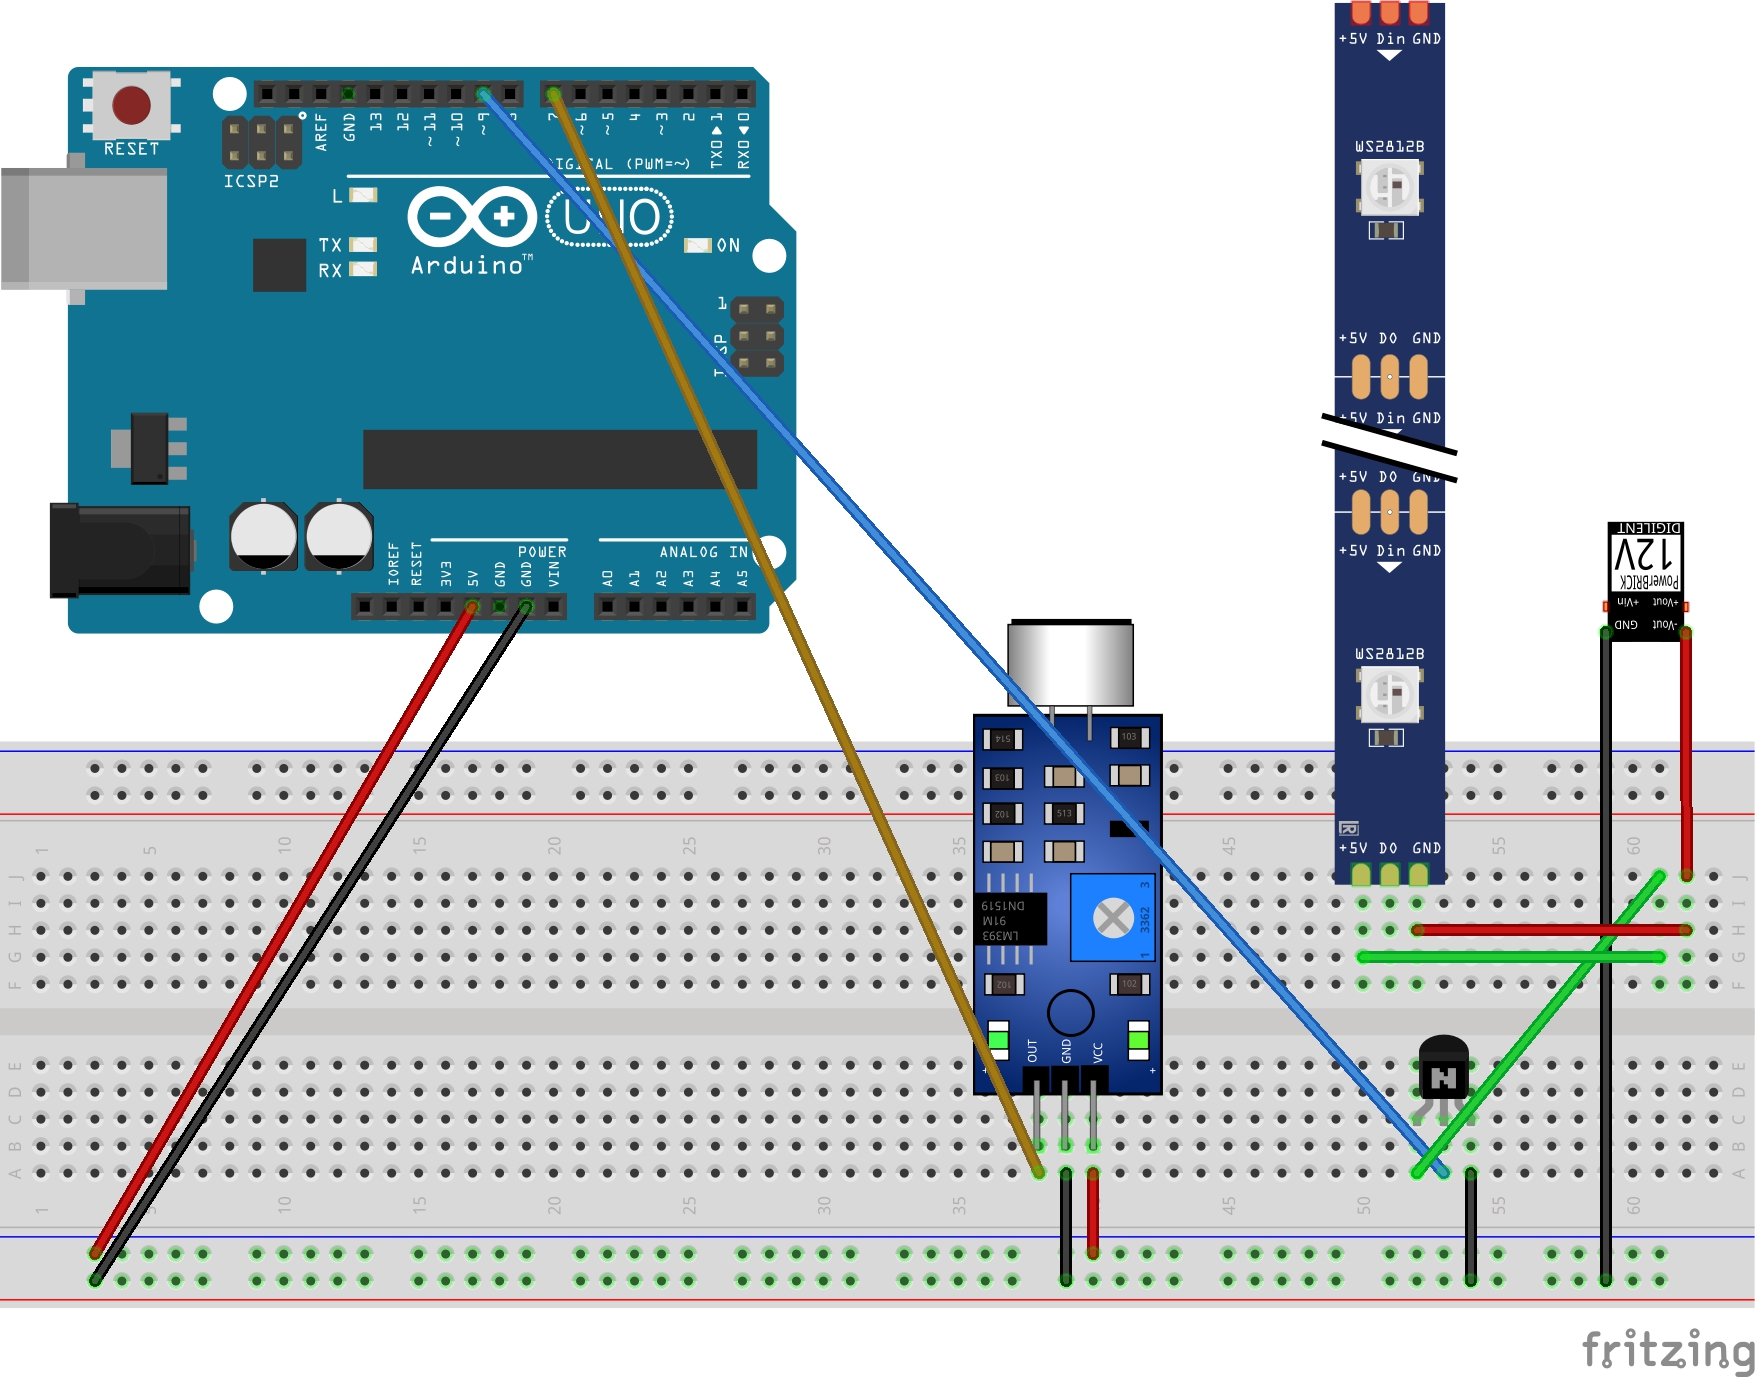
\includegraphics[width=0.66\textwidth]{Clapping_lamp_fritzing_bb.jpg}
\end{center}

\pagebreak

\subsection{Felhasznált kód}

\begin{lstlisting}[basicstyle=\small]
int ledPin=9;
int sensorPin=7;

boolean status_lights = false;

// for counting and calibrating clap
int clap = 0;
long detection_range_start = 0;
long detection_range = 0;

void setup(){
  pinMode(ledPin, OUTPUT);
  pinMode(sensorPin, INPUT);
}
  
void loop (){
  int status_sensor = digitalRead(sensorPin); // sound sensor HIGH or LOW
  
  if (status_sensor == 1){
    if (clap == 0){
      detection_range_start = detection_range = millis();
      clap++; 
    } else if (clap > 0 && millis()-detection_range >= 100){
      detection_range = millis();
      clap++;
    }
  }
  
  if (millis()-detection_range_start >= 600){
    if (clap == 2){ 
      if (!status_lights){
        digitalWrite(ledPin, HIGH);
        status_lights = true;
        clap = 0;
      } else if (status_lights){
        status_lights = false;
        digitalWrite(ledPin, LOW);
      }
    }
    clap = 0;
  }
}
\end{lstlisting} 

\section{Tapasztalat}

Elég szórakoztató használni és szerintem viszonylag jól be kallibráltam az adott környezetre, de később érdemes lesz tovább fejleszteni, mert a valós életben sokszor előfordulhat olyan környezeti zaj, amire a hangdetektor érzékeny. Szóval esetleg egy nem annyira jellegzetes 2 rövid 1 hosszú szünet a tapsok között, így lehet célnak megfelelőbben működne.

\vspace{0.5cm}
	
\begin{center}
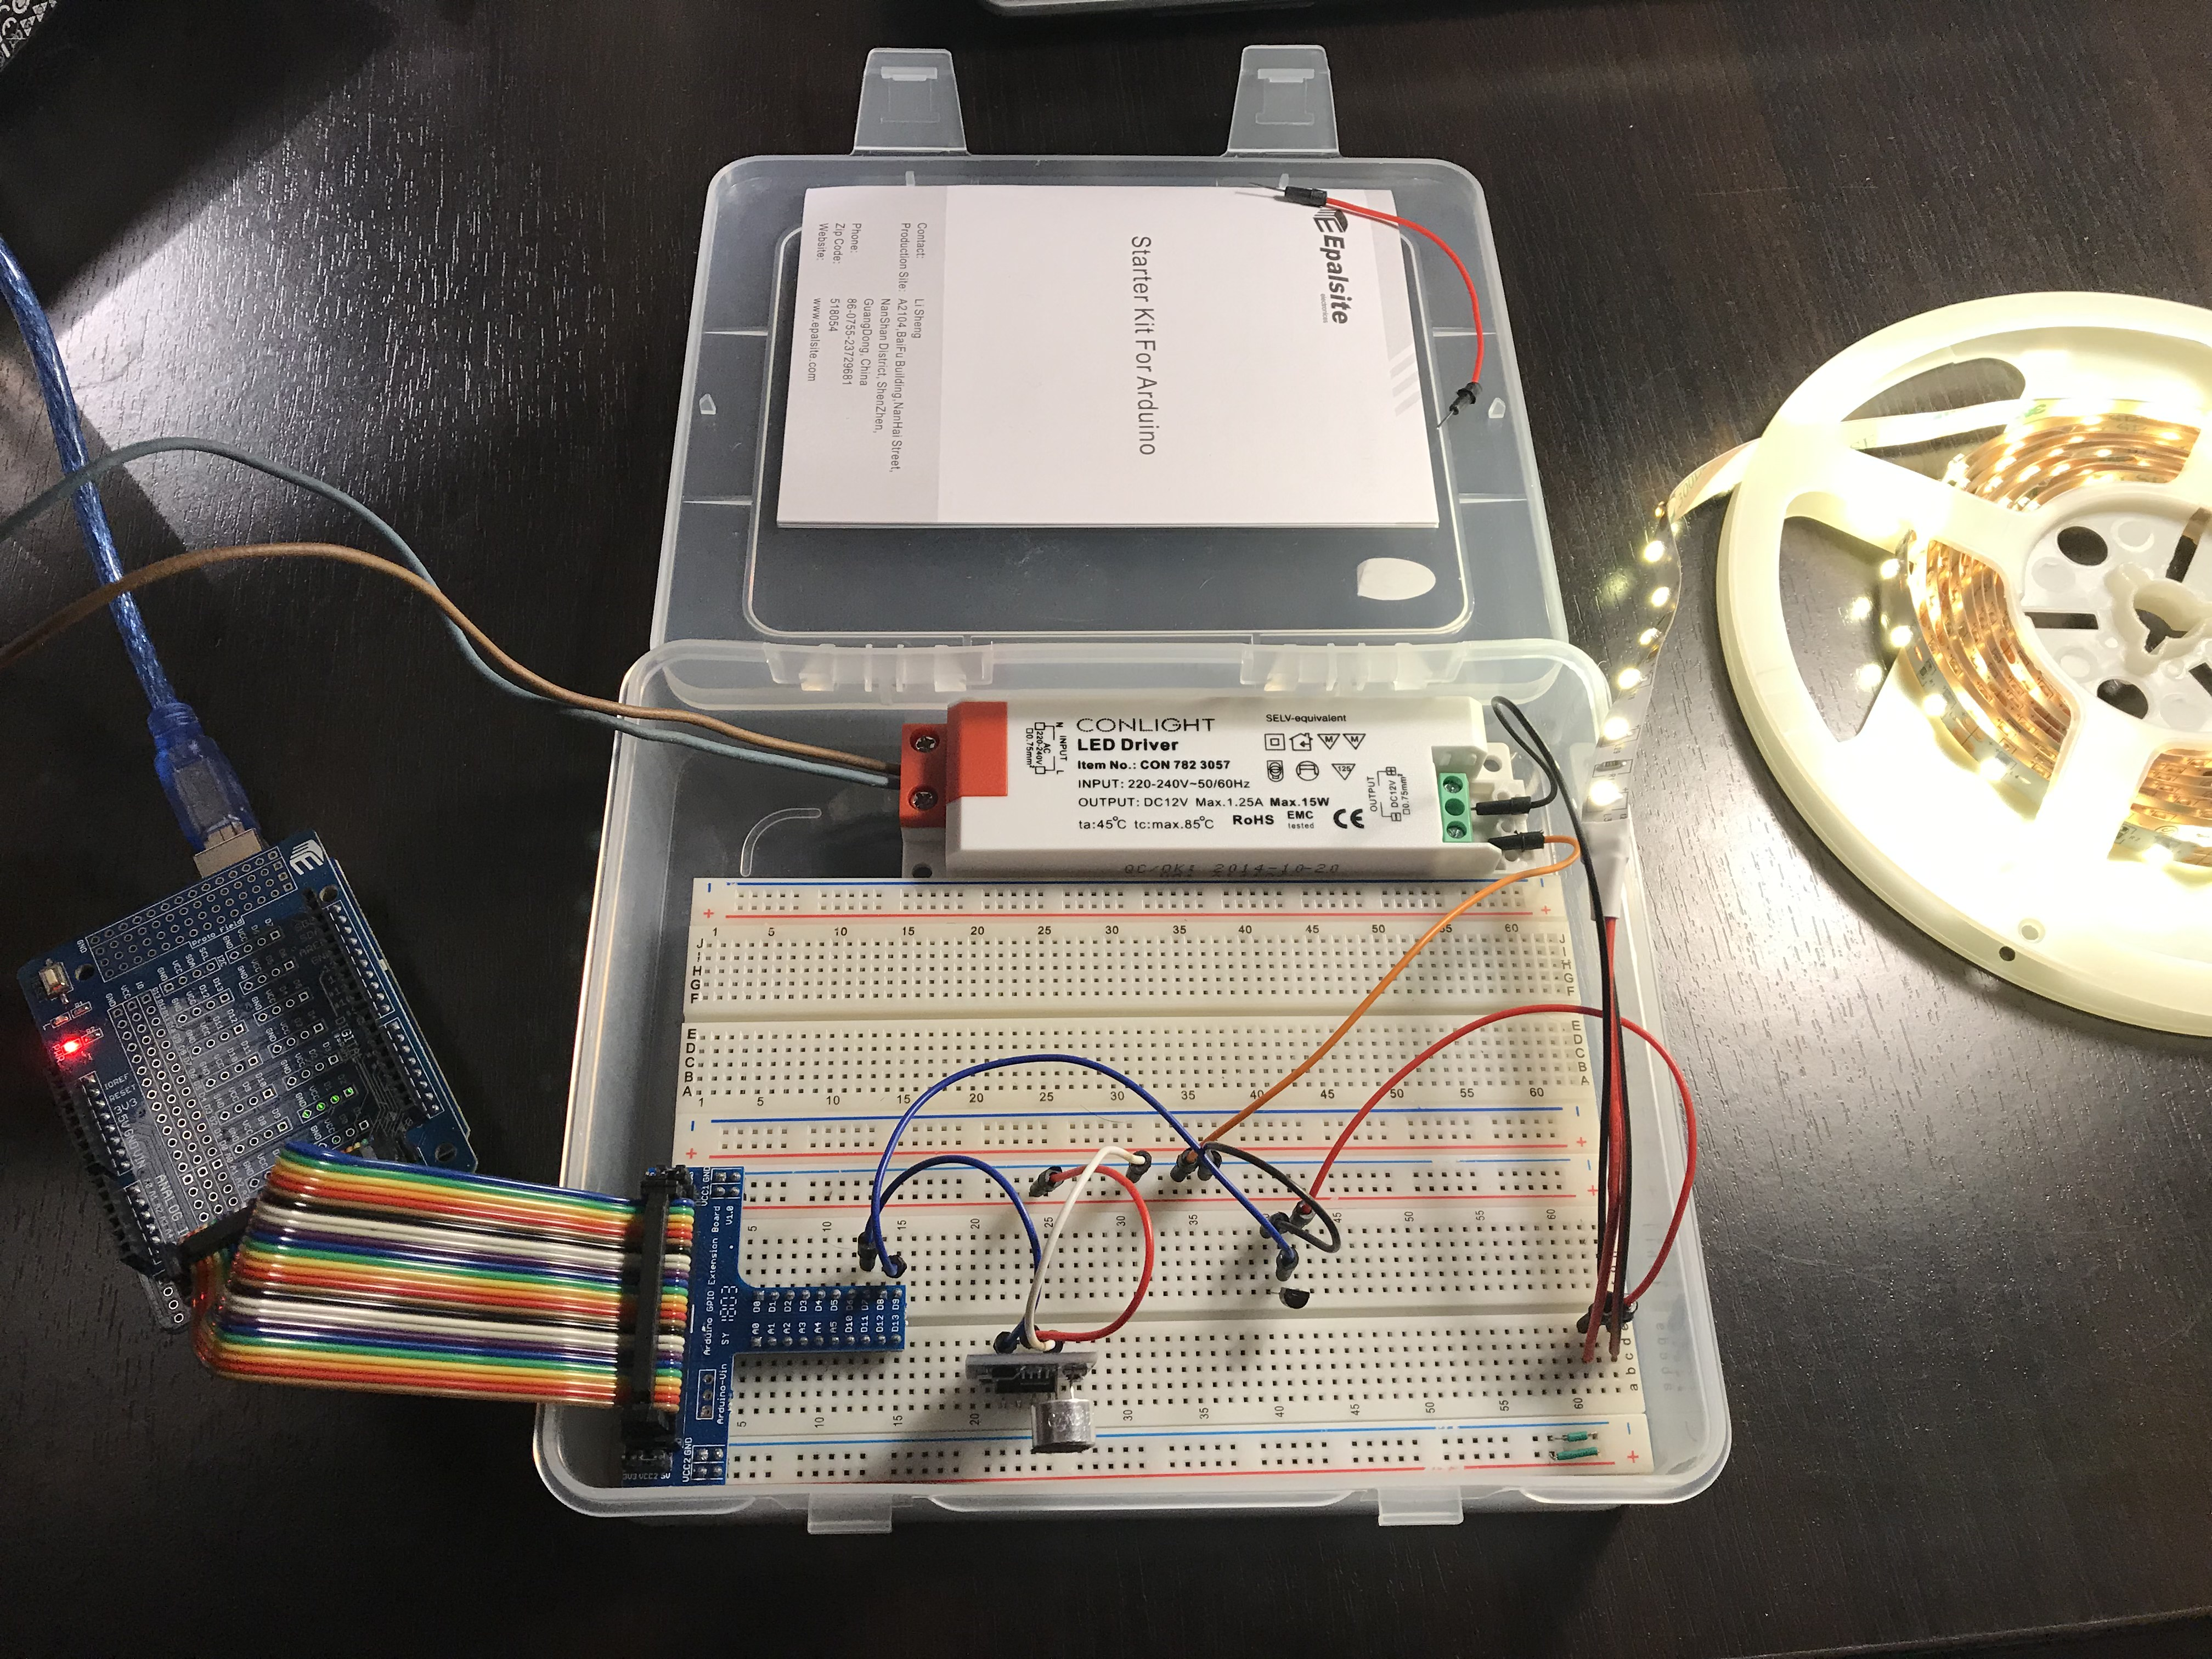
\includegraphics[width=0.36\textwidth]{clapping_lamp_on.jpeg}
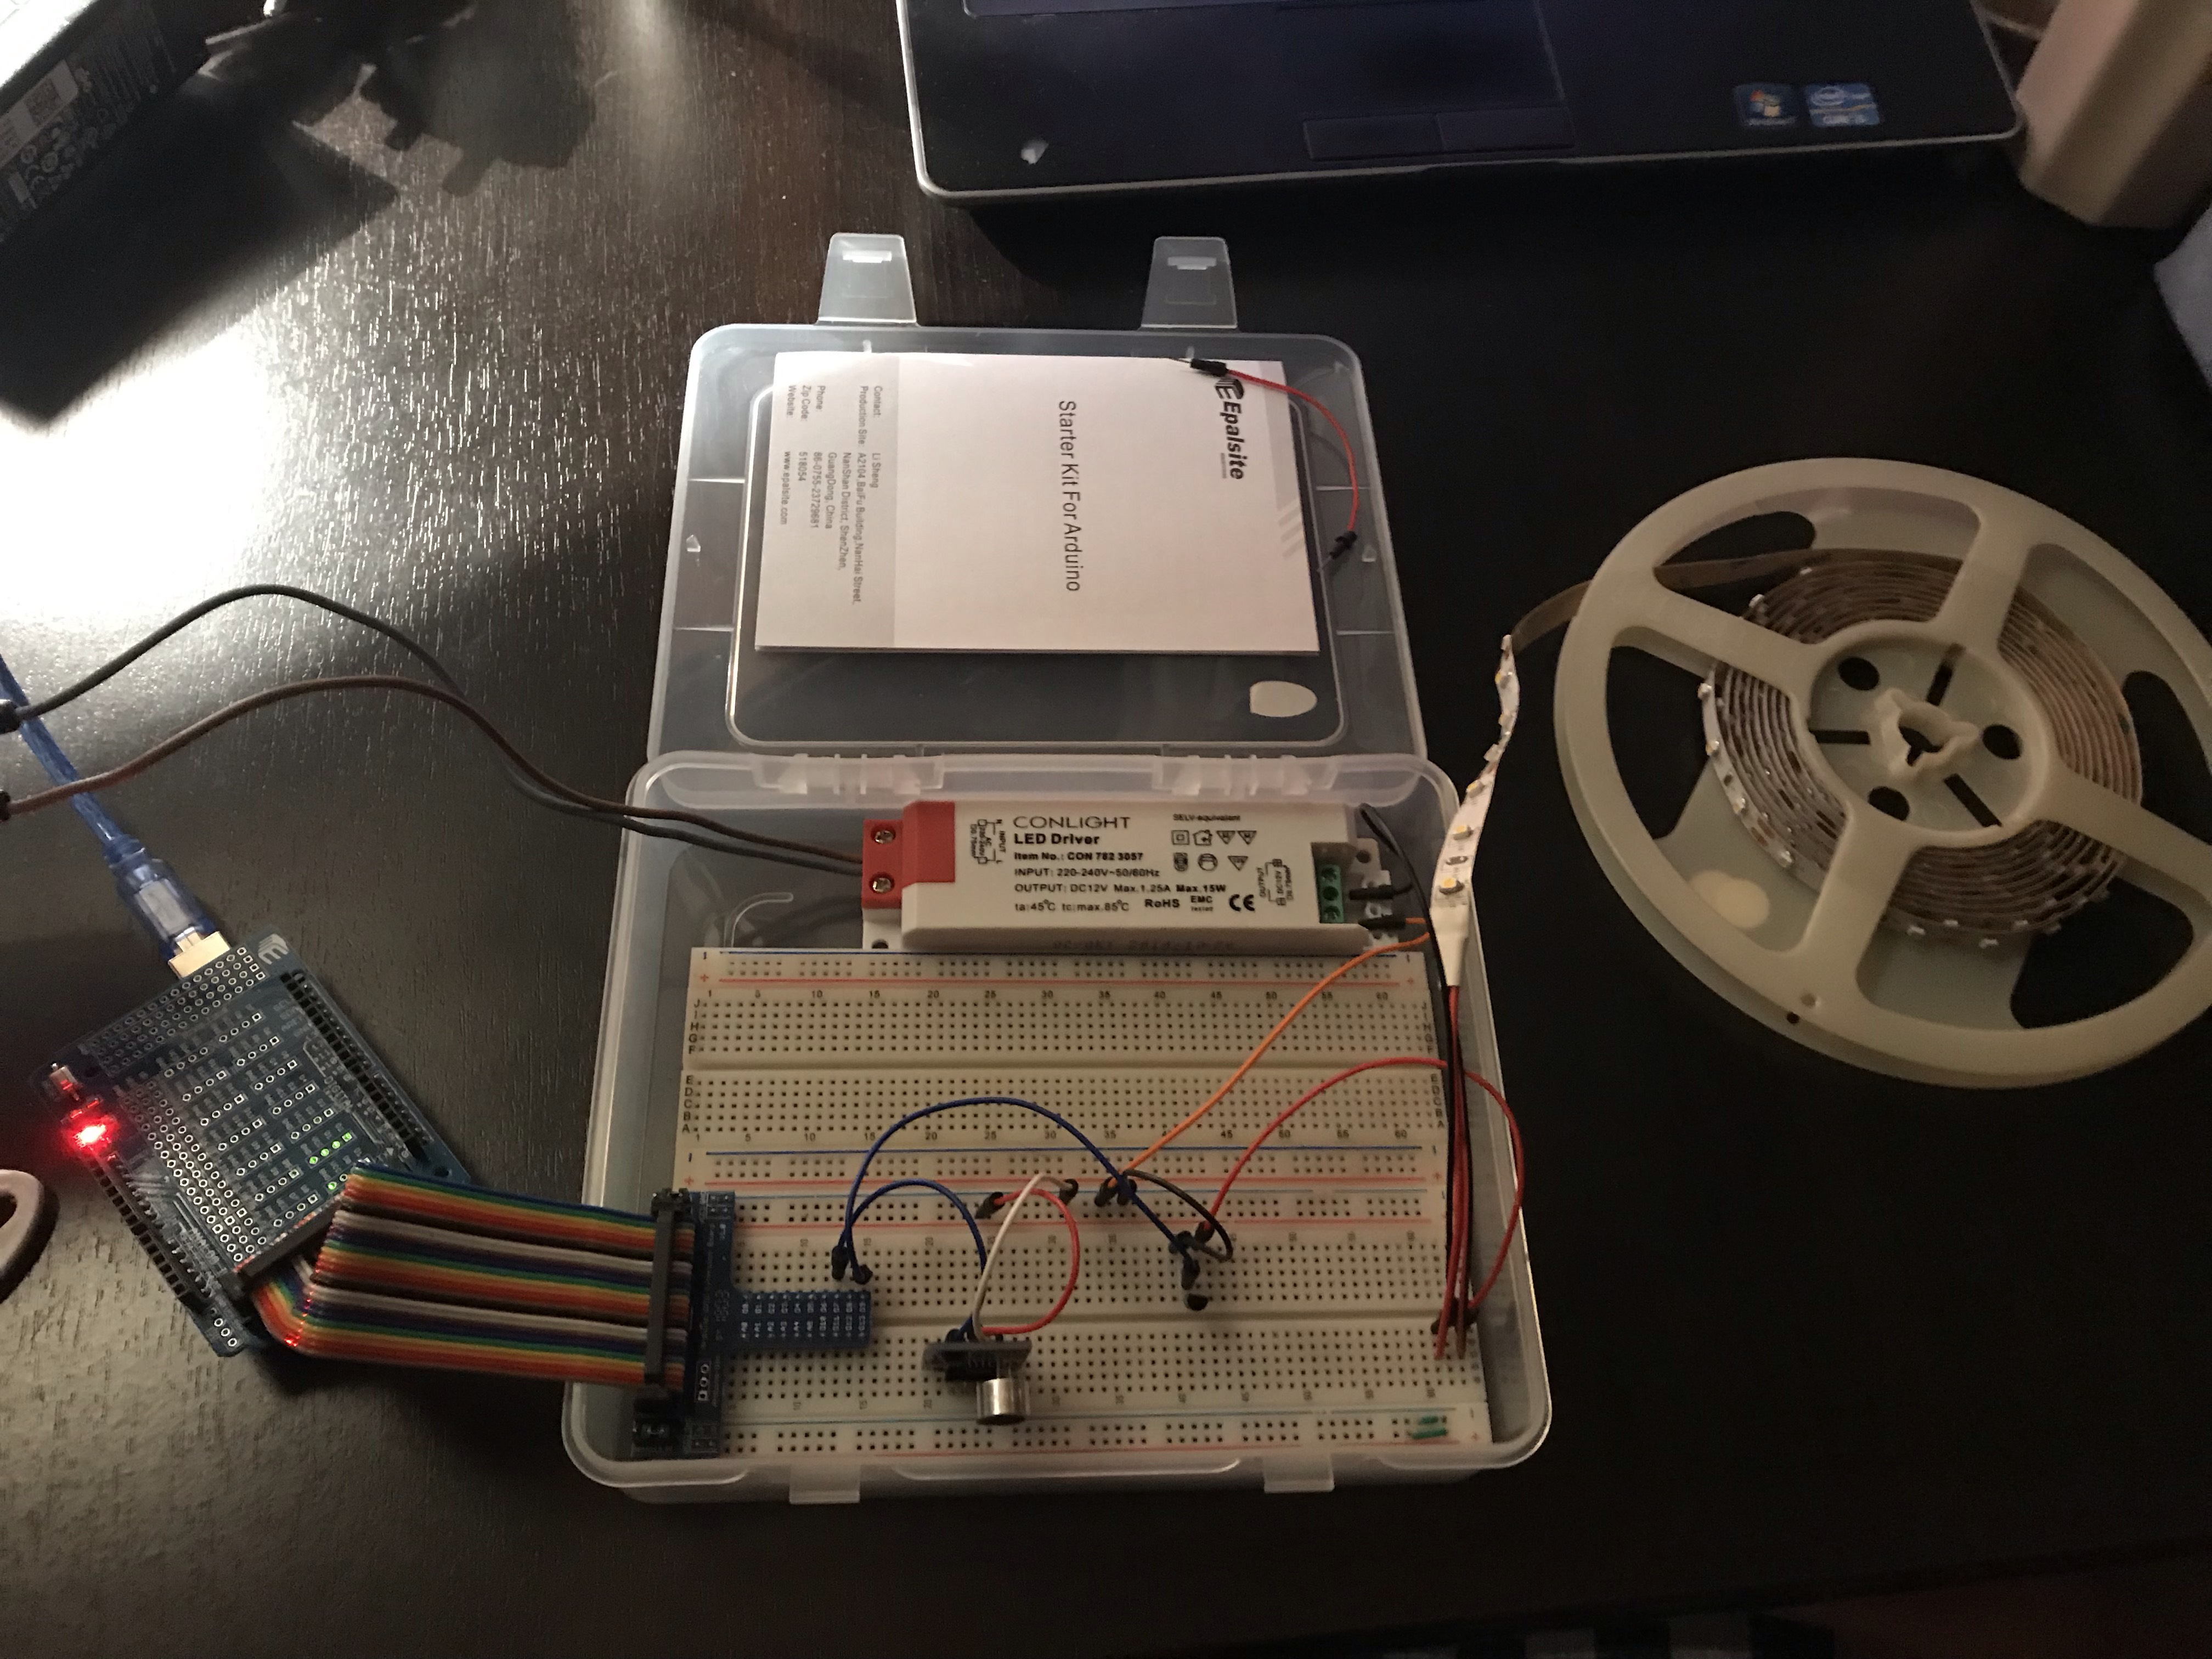
\includegraphics[width=0.36\textwidth]{clapping_lamp_off.jpg}
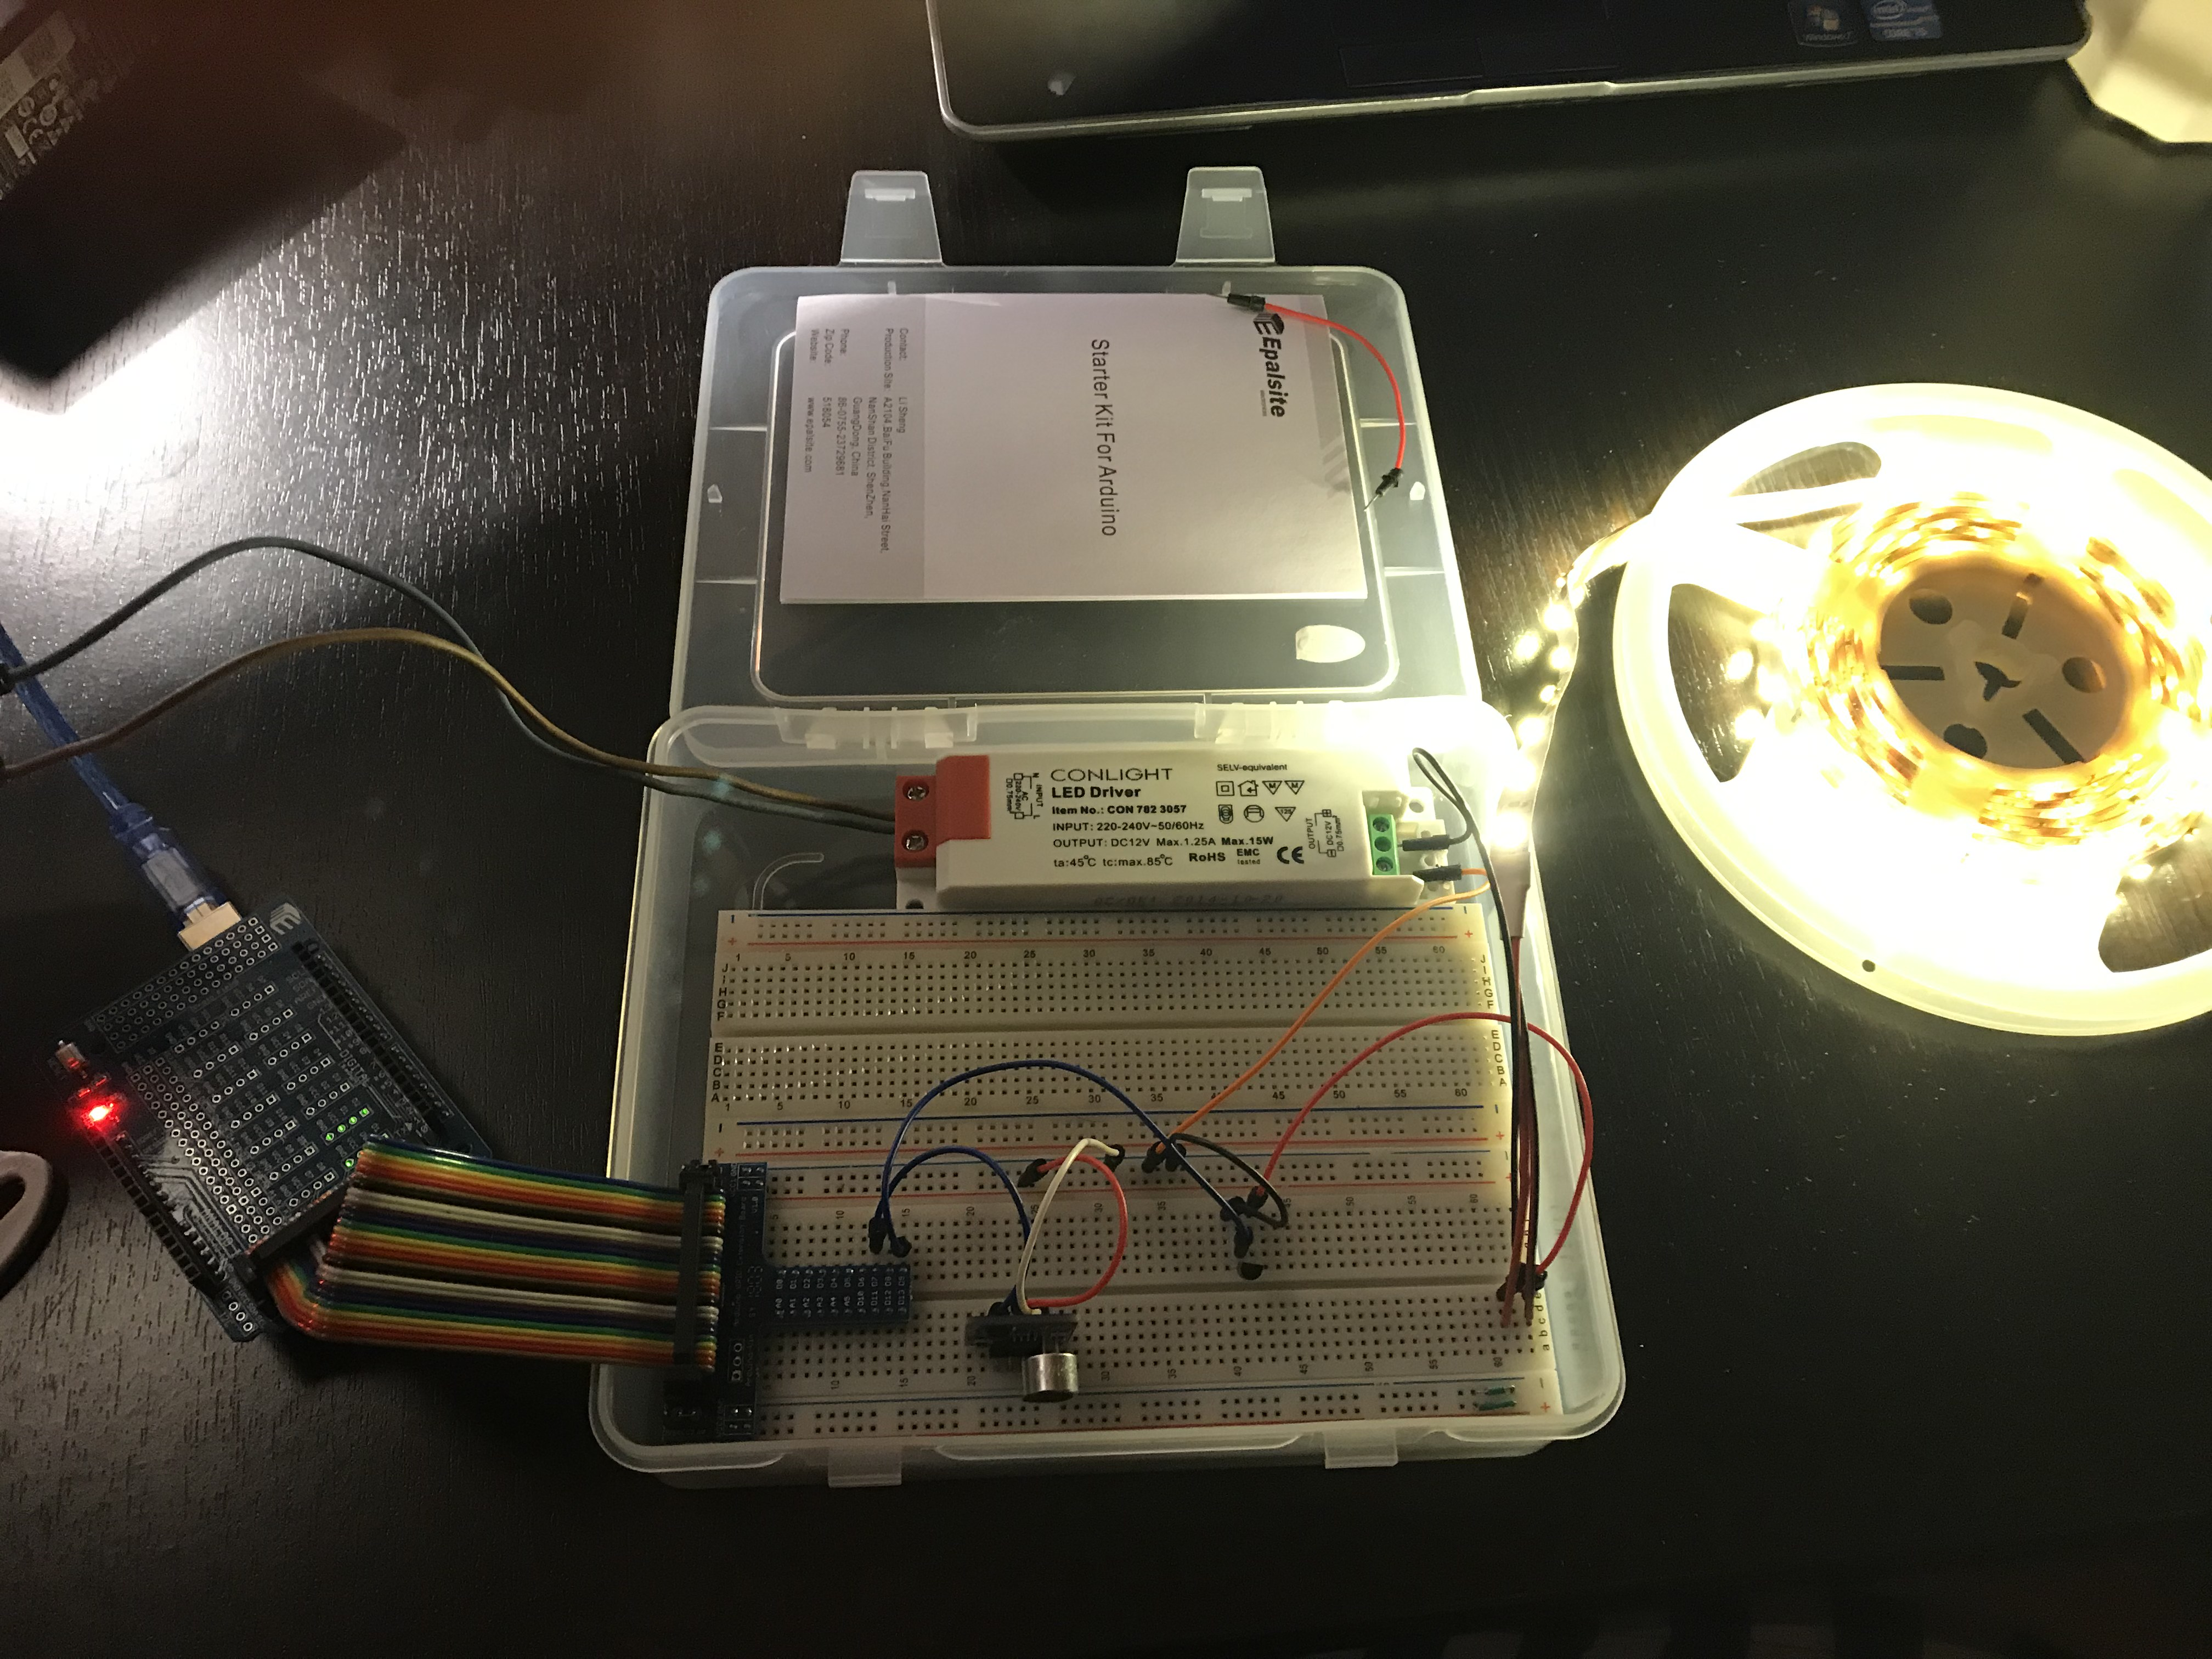
\includegraphics[width=0.729\textwidth]{clapping_lamp_full.jpeg}
\end{center}
\end{document}